\chapter{Advanced Class Modeling \\
  \small{\textit{-- Evan Ciok, Sophia DiCuffa, Carson McManus}}
  \index{Chapter!labtwo}
  \index{Lab Two}
  \label{Chapter::LabTwo}}

% Add a section and label it so that we can reference it later
\section{Advanced Class Modeling \label{Section::LabTwo}}

\subsection{Exercise 3.1}

\begin{itemize}
  \item Line Segment aggregates two points. A point can be a part of one or two line segments.
  \item A line is composed of any number of line segments. A line segment can only belong to one line.
  \item A sheet, buffer, and selection all aggregate any number of lines and boxes.
  \item Any number of lines links two boxes. A box can link any number of lines.
  \item Line or box can be a part of zero to one buffer, selection, and sheet.
\end{itemize}

\subsection{Exercise 3.2}

\begin{figure}
  \centering
  \scalebox{0.3}{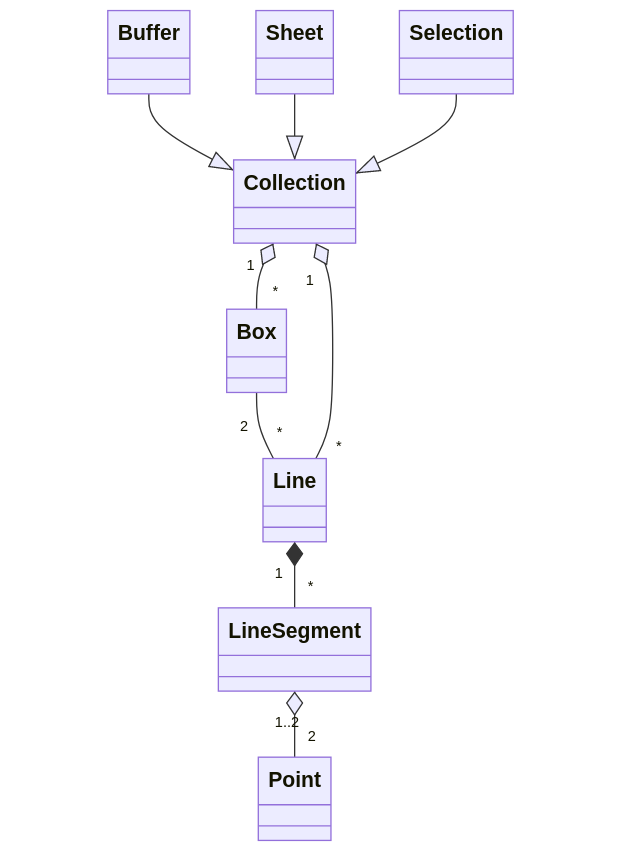
\includegraphics{Figures/lab2/uml.png}}
  \caption{\label{Figure::lab2uml} Revised class diagram.}
\end{figure}

The revision generalizes the interface that is used to put boxes and lines into a collection. It makes
the diffrences more visually clear.
